% !TEX TS-program = pdflatex
% !TEX encoding = UTF-8 Unicode

% This file is a template using the "beamer" package to create slides for a talk or presentation
% - Giving a talk on some subject.
% - The talk is between 15min and 45min long.
% - Style is ornate.

% MODIFIED by Jonathan Kew, 2008-07-06
% The header comments and encoding in this file were modified for inclusion with TeXworks.
% The content is otherwise unchanged from the original distributed with the beamer package.

\documentclass{beamer}
\setbeamercovered{invisible}



% Copyright 2004 by Till Tantau <tantau@users.sourceforge.net>.
%
% In principle, this file can be redistributed and/or modified under
% the terms of the GNU Public License, version 2.
%
% However, this file is supposed to be a template to be modified
% for your own needs. For this reason, if you use this file as a
% template and not specifically distribute it as part of a another
% package/program, I grant the extra permission to freely copy and
% modify this file as you see fit and even to delete this copyright
% notice. 


\mode<presentation>
{
  \usetheme{Warsaw}
  % or ...

  % or whatever (possibly just delete it)
}


\usepackage[english]{babel}
% or whatever

\usepackage[utf8]{inputenc}
\usepackage{qrcode}
\usepackage{hyperref}
\usepackage{ytableau}
\usepackage{tikz}
% or whatever

\usepackage{times}
\usepackage[T1]{fontenc}
% Or whatever. Note that the encoding and the font should match. If T1
% does not look nice, try deleting the line with the fontenc.

%%% MATH RELATED
\newcommand{\N}{\mathbb{N}}
\newcommand{\Z}{\mathbb{Z}}
\newcommand{\R}{\mathbb{R}}
\newcommand{\pow}{\mathcal{P}}


% All Venn diagrams are editable TikZ artwork.
\newcommand{\vennbase}{
 \draw[thick] (-2.7,-1.65) rectangle (2.7,1.65);
 \draw[thick] (-.8,0) circle (1.2);
 \draw[thick] (.8,0) circle (1.2);
 \node at (-1.45,1.25) {$A$}; \node at (1.45,1.25) {$B$};
 \node at (-2.4,1.38) {$U$};}
\newcommand{\venn}[1]{\begin{tikzpicture}[scale=.9]
 \ifcase#1\relax
 \or \fill[blue!25] (-.8,0) circle (1.2);\fill[blue!25] (.8,0) circle (1.2);
 \or \begin{scope}\clip (-.8,0) circle (1.2);\fill[blue!35] (.8,0) circle (1.2);\end{scope}
 \or \fill[blue!30] (-.8,0) circle (1.2);\begin{scope}\clip (.8,0) circle (1.2);\fill[white] (-.8,0) circle (1.2);\end{scope}
 \or \fill[blue!25] (-2.7,-1.65) rectangle (2.7,1.65);\fill[white] (-.8,0) circle (1.2);
 \or \fill[blue!25] (-2.7,-1.65) rectangle (2.7,1.65);\fill[white] (-.8,0) circle (1.2);\fill[white] (.8,0) circle (1.2);
 \or \fill[blue!25] (-2.7,-1.65) rectangle (2.7,1.65);\begin{scope}\clip (-.8,0) circle (1.2);\fill[white] (.8,0) circle (1.2);\end{scope}
 \fi
 \vennbase
 \end{tikzpicture}}
\newcommand{\histsource}[2]{\par\medskip{\tiny Source: \href{#1}{#2}.\par}}

\title{MATH 180 Strategies of Problem Solving} 
\subtitle
{} % (optional)

\author[W.R. Casper] % (optional, use only with lots of authors)
{W.R. Casper}
% - Use the \inst{?} command only if the authors have different
%   affiliation.

\institute[California State University Fullerton] % (optional, but mostly needed)
{
  Department of Mathematics\\
  California State University Fullerton}
% - Use the \inst command only if there are several affiliations.
% - Keep it simple, no one is interested in your street address.

\subject{Talks}
% This is only inserted into the PDF information catalog. Can be left
% out. 



% If you have a file called "university-logo-filename.xxx", where xxx
% is a graphic format that can be processed by latex or pdflatex,
% resp., then you can add a logo as follows:

% \pgfdeclareimage[height=0.5cm]{university-logo}{university-logo-filename}
% \logo{\pgfuseimage{university-logo}}



% Delete this, if you do not want the table of contents to pop up at
% the beginning of each subsection:
\AtBeginSubsection[]
{
  \begin{frame}<beamer>{Outline}
    \tableofcontents[currentsection,currentsubsection]
  \end{frame}
}


% If you wish to uncover everything in a step-wise fashion, uncomment
% the following command: 

%\beamerdefaultoverlayspecification{<+->}


\begin{document}

\begin{frame}
  \titlepage
\end{frame}

\begin{frame}{Outline}
  \tableofcontents
  % You might wish to add the option [pausesections]
\end{frame}

% Since this a solution template for a generic talk, very little can
% be said about how it should be structured. However, the talk length
% of between 15min and 45min and the theme suggest that you stick to
% the following rules:  

% - Exactly two or three sections (other than the summary).
% - At *most* three subsections per section.
% - Talk about 30s to 2min per frame. So there should be between about
%   15 and 30 frames, all told.

\section{SoPS Lecture 18}

\subsection{Counting and power sets}
\begin{frame}{Cardinality}
\begin{block}{Definition for finite sets}
The \textbf{cardinality} $|A|$ is the number of elements of $A$.
\end{block}\[|\{2,4,6\}|=3,\qquad|\varnothing|=0,\qquad|\{\varnothing\}|=1.\]
\begin{block}{Counting overlap}
For finite sets,\[|A\cup B|=|A|+|B|-|A\cap B|.\]The subtraction corrects the elements counted in both sets.
\end{block}
\end{frame}
\begin{frame}{How many elements?}
Count the objects at the outermost level of braces.
\begin{block}{Discuss with a partner}
\begin{itemize}
\item $|\{1,1,2\}|$
\item $|\{\varnothing,\{\varnothing\}\}|$
\item $|\{\{1,2,3\}\}|$
\item $|\{1,\{1\},\{\{1\}\}\}|$
\end{itemize}
\end{block}
\end{frame}
\begin{frame}{How many elements? --- discussion}
Count the objects at the outermost level of braces.
\begin{itemize}
\item $2$: the elements are $1$ and $2$.
\item $2$: the empty set and a singleton are distinct.
\item $1$: the one element is the set $\{1,2,3\}$.
\item $3$: each successive pair of braces creates a different object.
\end{itemize}
\end{frame}
\begin{frame}{Inclusion-Exclusion Principle}
\begin{block}{Two sets}
\[|A\cup B|=|A|+|B|-|A\cap B|.\]
\end{block}
\begin{block}{Three sets}
\[|A\cup B\cup C|=|A|+|B|+|C|-|A\cap B|-|A\cap C|-|B\cap C|+|A\cap B\cap C|.\]
\end{block}
\begin{block}{$n$ sets}
\[|A_1\cup A_2\cup\dots \cup A_n|=\sum_{k=1}^n|A_k|-\sum_{j<k}|A_j\cap A_k|+\sum_{i < j < k} |A_i\cap A_j\cap A_k|-\dots\]
\end{block}
\end{frame}
\begin{frame}{The power set}
\begin{block}{Definition}
The \textbf{power set} $\pow(A)$ is the set of all subsets of $A$:\[\pow(A)=\{B:B\subseteq A\}.\]
\end{block}If $A=\{a,b\}$, then\[\pow(A)=\{\varnothing,\{a\},\{b\},\{a,b\}\}.\]\medskip Every element of $\pow(A)$ is itself a set.
\end{frame}
\begin{frame}{Counting all subsets}
If $A$ has $n$ elements, then\[|\pow(A)|=2^n.\]\begin{block}{Why?}
To choose a subset, make one of two choices for each element of $A$: include it or leave it out.
\end{block}\begin{itemize}
\item The empty set corresponds to leaving everything out.
\item $A$ itself corresponds to including everything.
\item List the eight subsets of $\{a,b,c\}$.
\end{itemize}
\end{frame}
\begin{frame}{Counting all subsets --- list}
\[\begin{aligned}\pow(\{a,b,c\})=\{&\varnothing,\\&\{a\},\{b\},\{c\},\\&\{a,b\},\{a,c\},\{b,c\},\\&\{a,b,c\}\}.\end{aligned}\]\medskip There are $1+3+3+1=8=2^3$ subsets.
\end{frame}
\begin{frame}{Power-set check}
Let $A=\{1,2\}$.
\begin{block}{Discuss with a partner}
\begin{itemize}
\item $1\in\pow(A)$
\item $\{1\}\in\pow(A)$
\item $\varnothing\in\pow(A)$ and $A\in\pow(A)$
\item $\{\{1\}\}\subseteq\pow(A)$
\end{itemize}
\end{block}
\end{frame}
\begin{frame}{Power-set check --- discussion}
Let $A=\{1,2\}$.
\begin{itemize}
\item False: $1$ is not a subset of $A$ under our convention.
\item True: $\{1\}\subseteq A$.
\item Both true: $\varnothing\subseteq A$ and $A\subseteq A$.
\item True: its only element $\{1\}$ belongs to $\pow(A)$.
\end{itemize}
\end{frame}
\begin{frame}{The power set of the empty set}
\[\pow(\varnothing)=\{\varnothing\}.\]\begin{block}{Reason}
The empty set has exactly one subset: itself.
\end{block}\[\pow(\{\varnothing\})=\{\varnothing,\{\varnothing\}\}.\]\begin{block}{Check}
What are the cardinalities of these two power sets?\medskip\par They are $1$ and $2$.
\end{block}
\end{frame}

\subsection{Ordered pairs and products}
\begin{frame}{Ordered pairs}
An \textbf{ordered pair} $(a,b)$ records a first entry and a second entry.\[(a,b)=(c,d)\quad\Longleftrightarrow\quad a=c\text{ and }b=d.\]\begin{itemize}
\item $(1,2)\ne(2,1)$.
\item $\{1,2\}=\{2,1\}$.
\item $(1,1)$ has two entries, while $\{1,1\}=\{1\}$ has one element.
\end{itemize}\medskip A pair of dice rolls records order. A set of observed values forgets it.
\end{frame}
\begin{frame}{Cartesian products}
\begin{block}{Definition}
$A\times B=\{(a,b):a\in A\text{ and }b\in B\}$.
\end{block}If $A=\{1,2\}$ and $B=\{a,b\}$,\[A\times B=\{(1,a),(1,b),(2,a),(2,b)\}.\]\begin{itemize}
\item For finite sets, $|A\times B|=|A|\,|B|$.
\item For two dice, the outcome set is $\{1,\ldots,6\}\times\{1,\ldots,6\}$.
\item There are $36$ ordered outcomes.
\end{itemize}
\end{frame}
\begin{frame}{Product check}
Let $A=\{1,2\}$ and $B=\{3\}$.
\begin{block}{Discuss with a partner}
\begin{itemize}
\item $(1,3)\in A\times B$
\item $\{1,3\}\in A\times B$
\item $A\times B=B\times A$
\item $A\times\varnothing=\varnothing$
\end{itemize}
\end{block}
\end{frame}
\begin{frame}{Product check --- discussion}
Let $A=\{1,2\}$ and $B=\{3\}$.
\begin{itemize}
\item True: $1\in A$ and $3\in B$.
\item False: the elements of the product are ordered pairs, not these unordered sets.
\item False: $(1,3)$ belongs only to the left side.
\item True: no second entry can come from the empty set.
\end{itemize}
\end{frame}
\subsection{Quantifiers and proofs}
\begin{frame}{For every and there exists}
\[\forall x\in A,\quad x\in B\]
means that every $x$ in $A$ belongs to $B$.
\medskip\par This is exactly $A\subseteq B$.
\[\exists x\in A\text{ such that }x\in B\]
means that at least one element belongs to both sets.
\medskip\par This is exactly $A\cap B\ne\varnothing$.
\end{frame}
\begin{frame}{What is missing?}
Which lines have a fixed truth value as written?
\begin{block}{Discuss with a partner}
\begin{itemize}
\item $x\in\{1,2\}$
\item $\forall x\in\{1,2\},\ x<3$
\item $\exists x\in\{1,2\},\ x>3$
\item $\{x\in\Z:x<3\}$
\end{itemize}
\end{block}
\end{frame}
\begin{frame}{What is missing? --- discussion}
Which lines have a fixed truth value as written?
\begin{itemize}
\item An open sentence: meaningful, but depends on $x$.
\item A true statement: check both $1$ and $2$.
\item A false statement: neither possible choice works.
\item A set expression, not a statement. The $x$ is bound inside the description.
\end{itemize}
\end{frame}
\section{Why is it called naive?}
\subsection{Russell's paradox}
\begin{frame}{When sets get too big}
So far, we have selected elements from an existing set:
\[\{x\in U:P(x)\}.\]
\begin{block}{Can sets get too big?}
Is there a set of \emph{everything}?
\end{block}
Consider the proposed set
\[U=\{S:S\text{ is a set}\}.\]
\end{frame}
\begin{frame}{Weirdness happens}
We can already detect some strangeness:
$$U\in U$$
$$\mathcal P(U)\in U$$
Consider the proposed set
\[R=\{S\in U:S\notin S\}.\]
$R$ is the set of all sets which are not elements of themselves.
\end{frame}
\begin{frame}{Russell's paradox}
Suppose $R=\{S:S\text{ is a set and }S\notin S\}$ were a set.\medskip\par Does $R\in R$?\begin{itemize}
\item If $R\in R$, then $R$ must satisfy the defining condition, so $R\notin R$.
\item If $R\notin R$, then $R$ satisfies the defining condition, so $R\in R$.
\end{itemize}\begin{block}{The conclusion}
This unrestricted description cannot define a set. The problem is the assumption that every condition produces a set.
\end{block}
\end{frame}
\begin{frame}{A barber's perspective}
\begin{center}
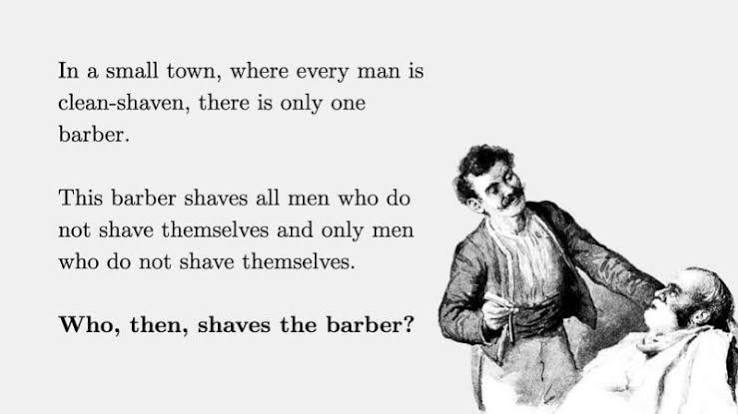
\includegraphics[width=\linewidth]{fig/barber}
\end{center}
\end{frame}
\begin{frame}{Why this mattered to Frege}
\begin{itemize}
\item Gottlob Frege sought to derive arithmetic from logic.
\item His \emph{Grundgesetze der Arithmetik} appeared in two volumes, in 1893 and 1903.
\item Its Basic Law V governed when two value-ranges are equal. Together with his logical system, it allowed the contradiction.
\item The issue reached the foundations of his project, rather than an isolated calculation.
\end{itemize}\histsource{https://bracers.mcmaster.ca/53946}{Russell Archives, letter of 16 June 1902 and editorial note}\histsource{https://www.tha.de/~harsch/germanica/Chronologie/19Jh/Frege/fre_brif.html}{Frege to Russell, 22 June 1902}
\end{frame}
\begin{frame}{Russell's wonderfully understated letter}
\begin{block}{16 June 1902}
``There is just one point where I have encountered a difficulty.''
\end{block}
Russell praises Frege's work, then explains that either answer to the self-membership question gives its opposite.
\medskip\par His conclusion: being describable does not guarantee that a collection forms a set.
\medskip\par \textbf{Check:} What assumption does our proof force us to reject?\histsource{https://bracers.mcmaster.ca/53946}{Russell to Frege, Woodward translation, Russell Archives}
\end{frame}
\begin{frame}{Frege receives the letter}
\begin{center}
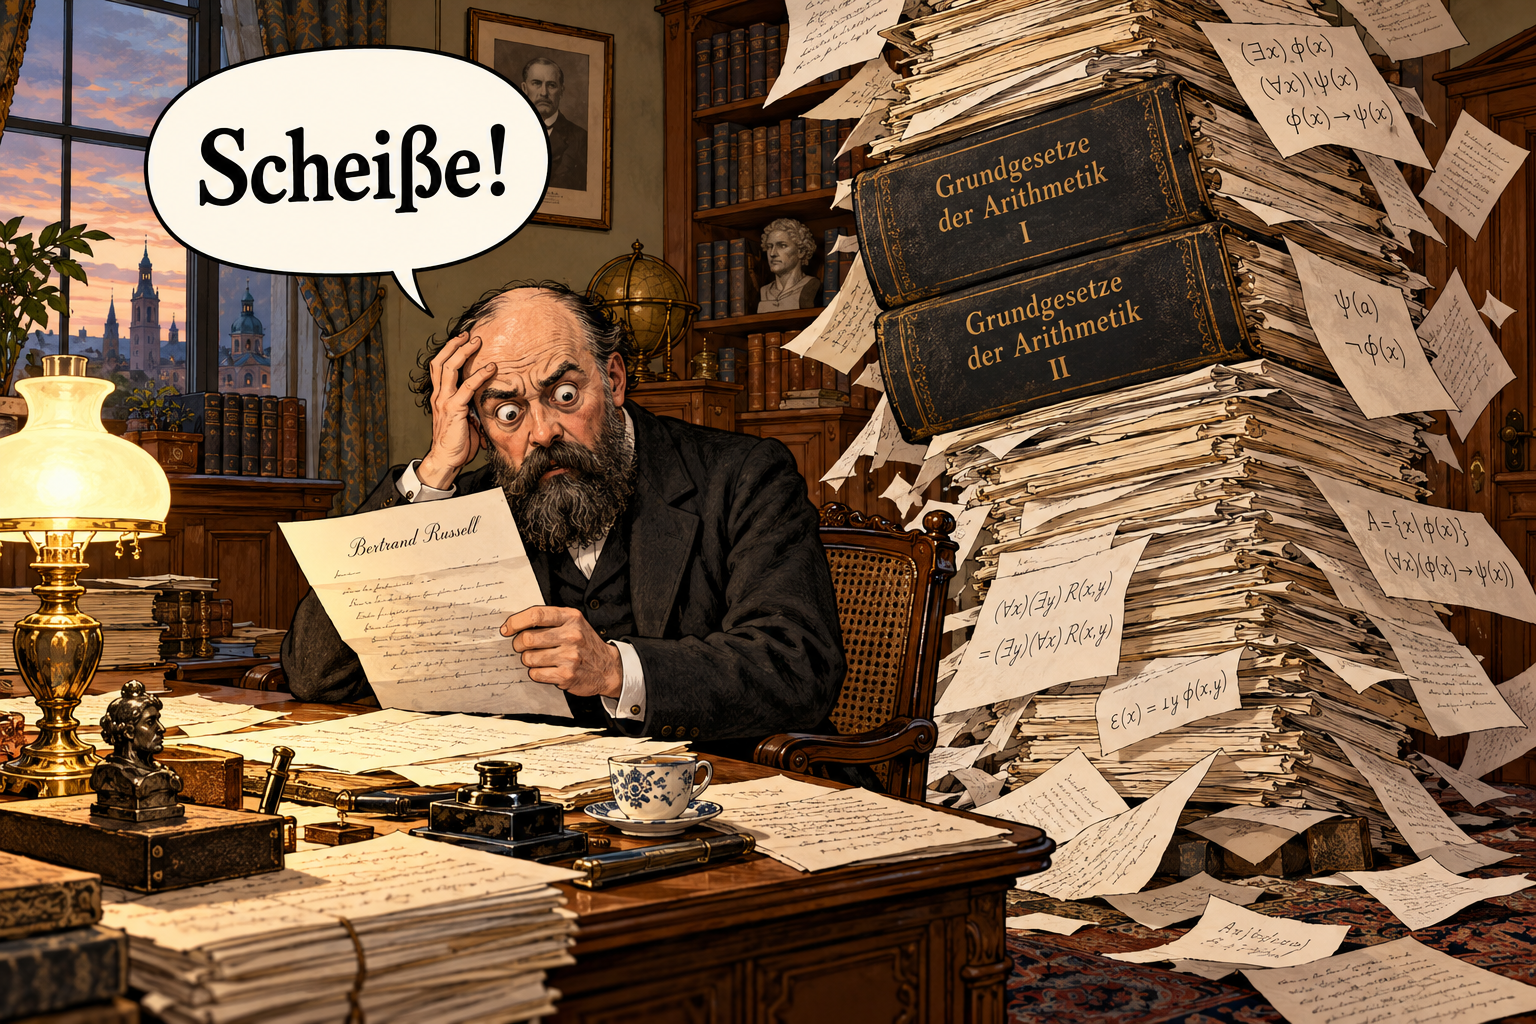
\includegraphics[width=.96\linewidth,height=.72\textheight,keepaspectratio]{fig/frege-russell-joke.png}
\end{center}
\centering\scriptsize Real footage of Friege reading Russell's letter that definitely wasn't AI-generated\par ``Schei\ss e!'' means ``hello!'' 
\end{frame}
\begin{frame}{Frege's reply: 22 June 1902}
\begin{block}{An actual reaction, in translation}
``Your discovery of the contradiction has surprised me beyond words''
\end{block}
Frege identifies Basic Law V as the source of the difficulty and worries about the foundations of arithmetic.
\medskip\par He also hopes the discovery may produce progress in logic and says he must think further about it.\histsource{https://www.cs.mcgill.ca/~dirk/80-110spring02/quotes.html}{Frege Reader, p. 254, excerpt reproduced by Dirk Schlimm}\histsource{https://www.tha.de/~harsch/germanica/Chronologie/19Jh/Frege/fre_brif.html}{Frege's original German letter}
\end{frame}
\begin{frame}{Timeline: the letter arrives}
\begin{description}
\item[1901] Russell discovers the contradiction.
\item[16 June 1902] He writes to Frege about it.
\item[22 June 1902] Frege replies and acknowledges the problem.
\item[1903] Frege publishes volume II with an appendix addressing the contradiction. Russell publishes \emph{The Principles of Mathematics}.
\end{description}\histsource{https://plato.stanford.edu/entries/russell-paradox/}{Russell's Paradox, historical discussion}\histsource{https://bracers.mcmaster.ca/53946}{Russell Archives, 53946}\histsource{https://www.tha.de/~harsch/germanica/Chronologie/19Jh/Frege/fre_brif.html}{Original correspondence}
\end{frame}
\begin{frame}{The real manuscript was already going to press}
\begin{itemize}
\item The second volume was nearing publication when the letter arrived.
\item Frege added an appendix explaining that a foundation of the finished work had been shaken.
\item He proposed a repair to Basic Law V. The repair did not successfully restore the intended foundation.
\item The cartoon exaggerates the scene. The admission in print was real.
\end{itemize}\histsource{https://bracers.mcmaster.ca/53946}{Russell Archives, editorial note quoting the appendix}\histsource{https://plato.stanford.edu/entries/russell-paradox/}{Frege's response}
\end{frame}
\begin{frame}{Hilbert's reaction: already known in Göttingen}
\begin{itemize}
\item On 7 November 1903, David Hilbert wrote to Frege after receiving volume II.
\item He reported that the contradiction was already known in G\"ottingen, and credited Ernst Zermelo with discovering it independently several years earlier.
\item For Hilbert, such problems called for clearer axioms and attention to consistency.
\end{itemize}\medskip The discovery did not reach everyone at the same time or have the same impact on every foundational project.\histsource{https://www.numdam.org/item/PHSC_2005__9_S2_199_0.pdf}{Volker Peckhaus, Pro and Contra Hilbert (2005), pp. 203--205}
\end{frame}
\begin{frame}{How mathematicians responded}
\begin{description}
\item[1908: Zermelo] An axiomatic set theory restricts set formation.
\item[1908: Russell] A theory of types controls which objects can apply to which others.
\item[1910--1913] Whitehead and Russell publish the three volumes of \emph{Principia Mathematica}.
\end{description}
\end{frame}
\begin{frame}{Two ways to block the construction}
\begin{block}{Axiomatic set theory: restrict set formation}
Select from an existing set $U$:
\[R_U=\{x\in U:x\notin x\}.\]
This set exists, but $R_U$ cannot belong to $U$.
\end{block}
\begin{block}{A simple type hierarchy: restrict expressions}
A set at one level has elements at a lower level. Self-membership $x\in x$ fails the type rules.
\end{block}
These approaches impose different rules for meaningful expressions.\histsource{https://sites.pitt.edu/~jdnorton/teaching/paradox/paradox_fall_2021/chapters/sets/sets.html}{John D. Norton, Naive Set Theory, type and axiomatic approaches}
\end{frame}
\begin{frame}{Why restricting to a universe helps}
Let $R_U=\{x\in U:x\notin x\}$.
\medskip\par Suppose $R_U\in U$. Then its defining condition gives
\[R_U\in R_U\quad\Longleftrightarrow\quad R_U\notin R_U,\]
which is impossible. Hence $R_U\notin U$.
\begin{block}{What follows?}
Every proposed set $U$ misses at least one set. There is no set of all sets in this axiomatic framework.
\end{block}
We can select within $U$ without assuming $U$ contains everything.
\end{frame}
\begin{frame}{Paradox check: what is the conclusion?}
\begin{itemize}
\item ``All mathematics is false.
\item ``The proposed set $R$ exists, but its membership is mysterious.
\item ``Unrestricted set formation leads to a contradiction.
\item ``Every discussion of self-reference is meaningless.
\end{itemize}\medskip Which conclusion does our argument justify?
\end{frame}
\begin{frame}{Paradox check --- discussion}
The argument justifies the third claim: unrestricted set formation leads to a contradiction.
\medskip\par It does not establish that all mathematics is false, or give us a mysterious existing set $R$.
\medskip\par Self-reference itself is not always meaningless. Its status depends on the language and rules we choose.
\begin{block}{Connection to our first questions}
We must distinguish a meaningful formula, an existence claim, and a construction our rules actually permit.
\end{block}
\end{frame}
\begin{frame}{Historical sources}
\small
\begin{itemize}
\item \href{https://bracers.mcmaster.ca/53946}{Russell to Frege, 16 June 1902}. Russell Archives, McMaster University, transcription and translation.
\item \href{https://www.tha.de/~harsch/germanica/Chronologie/19Jh/Frege/fre_brif.html}{Frege to Russell, 22 June 1902}. Original German, Bibliotheca Augustana.
\item \href{https://plato.stanford.edu/entries/russell-paradox/}{Russell's Paradox}. Stanford Encyclopedia of Philosophy, especially historical sections.
\item \href{https://www.numdam.org/item/PHSC_2005__9_S2_199_0.pdf}{V. Peckhaus, Pro and Contra Hilbert: Zermelo's Set Theories} (2005), pp. 203--205.
\item \href{https://sites.pitt.edu/~jdnorton/teaching/paradox/paradox_fall_2021/chapters/sets/sets.html}{J. D. Norton, Naive Set Theory}. Frege's appendix and foundational responses.
\end{itemize}
\end{frame}

\begin{frame}{What if we want all sets?}
\begin{itemize}
\item Naive set theory is still often fine...
\item What if we \emph{do} want to work with all sets?
\end{itemize}
We use \textbf{category theory}.\\
We can use the \textbf{category of all sets}, which has strong rules for how you can interact with it.\\
\medskip
Has its own foundational issues ... need \textit{Grothendieck universes}...
\end{frame}



\begin{frame}{Final thoughts}
  \begin{block}{Reflection}
\begin{itemize}
\item Describe Russell's paradox in your own words.  What did this mean for the development of set theory?
\end{itemize}
  \end{block}
\begin{center}
Submit your responses by \textbf{Tonight!}
\end{center}
\end{frame}


\end{document}


